% Options for packages loaded elsewhere
\PassOptionsToPackage{unicode}{hyperref}
\PassOptionsToPackage{hyphens}{url}
%
\documentclass[
  man]{apa6}
\usepackage{amsmath,amssymb}
\usepackage{lmodern}
\usepackage{iftex}
\ifPDFTeX
  \usepackage[T1]{fontenc}
  \usepackage[utf8]{inputenc}
  \usepackage{textcomp} % provide euro and other symbols
\else % if luatex or xetex
  \usepackage{unicode-math}
  \defaultfontfeatures{Scale=MatchLowercase}
  \defaultfontfeatures[\rmfamily]{Ligatures=TeX,Scale=1}
\fi
% Use upquote if available, for straight quotes in verbatim environments
\IfFileExists{upquote.sty}{\usepackage{upquote}}{}
\IfFileExists{microtype.sty}{% use microtype if available
  \usepackage[]{microtype}
  \UseMicrotypeSet[protrusion]{basicmath} % disable protrusion for tt fonts
}{}
\makeatletter
\@ifundefined{KOMAClassName}{% if non-KOMA class
  \IfFileExists{parskip.sty}{%
    \usepackage{parskip}
  }{% else
    \setlength{\parindent}{0pt}
    \setlength{\parskip}{6pt plus 2pt minus 1pt}}
}{% if KOMA class
  \KOMAoptions{parskip=half}}
\makeatother
\usepackage{xcolor}
\IfFileExists{xurl.sty}{\usepackage{xurl}}{} % add URL line breaks if available
\IfFileExists{bookmark.sty}{\usepackage{bookmark}}{\usepackage{hyperref}}
\hypersetup{
  pdftitle={A survey of registration practices among observational researchers using preexisting datasets},
  pdfauthor={Robert T. Thibault1,5, Marton Kovacs2,6, Tom E. Hardwicke3, Alexandra Sarafoglou4, John P. A. Ioannidis4, \& Marcus R. Munafò1,7},
  pdflang={en-EN},
  pdfkeywords={keywords},
  hidelinks,
  pdfcreator={LaTeX via pandoc}}
\urlstyle{same} % disable monospaced font for URLs
\usepackage{graphicx}
\makeatletter
\def\maxwidth{\ifdim\Gin@nat@width>\linewidth\linewidth\else\Gin@nat@width\fi}
\def\maxheight{\ifdim\Gin@nat@height>\textheight\textheight\else\Gin@nat@height\fi}
\makeatother
% Scale images if necessary, so that they will not overflow the page
% margins by default, and it is still possible to overwrite the defaults
% using explicit options in \includegraphics[width, height, ...]{}
\setkeys{Gin}{width=\maxwidth,height=\maxheight,keepaspectratio}
% Set default figure placement to htbp
\makeatletter
\def\fps@figure{htbp}
\makeatother
\setlength{\emergencystretch}{3em} % prevent overfull lines
\providecommand{\tightlist}{%
  \setlength{\itemsep}{0pt}\setlength{\parskip}{0pt}}
\setcounter{secnumdepth}{-\maxdimen} % remove section numbering
% Make \paragraph and \subparagraph free-standing
\ifx\paragraph\undefined\else
  \let\oldparagraph\paragraph
  \renewcommand{\paragraph}[1]{\oldparagraph{#1}\mbox{}}
\fi
\ifx\subparagraph\undefined\else
  \let\oldsubparagraph\subparagraph
  \renewcommand{\subparagraph}[1]{\oldsubparagraph{#1}\mbox{}}
\fi
\newlength{\cslhangindent}
\setlength{\cslhangindent}{1.5em}
\newlength{\csllabelwidth}
\setlength{\csllabelwidth}{3em}
\newlength{\cslentryspacingunit} % times entry-spacing
\setlength{\cslentryspacingunit}{\parskip}
\newenvironment{CSLReferences}[2] % #1 hanging-ident, #2 entry spacing
 {% don't indent paragraphs
  \setlength{\parindent}{0pt}
  % turn on hanging indent if param 1 is 1
  \ifodd #1
  \let\oldpar\par
  \def\par{\hangindent=\cslhangindent\oldpar}
  \fi
  % set entry spacing
  \setlength{\parskip}{#2\cslentryspacingunit}
 }%
 {}
\usepackage{calc}
\newcommand{\CSLBlock}[1]{#1\hfill\break}
\newcommand{\CSLLeftMargin}[1]{\parbox[t]{\csllabelwidth}{#1}}
\newcommand{\CSLRightInline}[1]{\parbox[t]{\linewidth - \csllabelwidth}{#1}\break}
\newcommand{\CSLIndent}[1]{\hspace{\cslhangindent}#1}
\ifLuaTeX
\usepackage[bidi=basic]{babel}
\else
\usepackage[bidi=default]{babel}
\fi
\babelprovide[main,import]{english}
% get rid of language-specific shorthands (see #6817):
\let\LanguageShortHands\languageshorthands
\def\languageshorthands#1{}
% Manuscript styling
\usepackage{upgreek}
\captionsetup{font=singlespacing,justification=justified}

% Table formatting
\usepackage{longtable}
\usepackage{lscape}
% \usepackage[counterclockwise]{rotating}   % Landscape page setup for large tables
\usepackage{multirow}		% Table styling
\usepackage{tabularx}		% Control Column width
\usepackage[flushleft]{threeparttable}	% Allows for three part tables with a specified notes section
\usepackage{threeparttablex}            % Lets threeparttable work with longtable

% Create new environments so endfloat can handle them
% \newenvironment{ltable}
%   {\begin{landscape}\centering\begin{threeparttable}}
%   {\end{threeparttable}\end{landscape}}
\newenvironment{lltable}{\begin{landscape}\centering\begin{ThreePartTable}}{\end{ThreePartTable}\end{landscape}}

% Enables adjusting longtable caption width to table width
% Solution found at http://golatex.de/longtable-mit-caption-so-breit-wie-die-tabelle-t15767.html
\makeatletter
\newcommand\LastLTentrywidth{1em}
\newlength\longtablewidth
\setlength{\longtablewidth}{1in}
\newcommand{\getlongtablewidth}{\begingroup \ifcsname LT@\roman{LT@tables}\endcsname \global\longtablewidth=0pt \renewcommand{\LT@entry}[2]{\global\advance\longtablewidth by ##2\relax\gdef\LastLTentrywidth{##2}}\@nameuse{LT@\roman{LT@tables}} \fi \endgroup}

% \setlength{\parindent}{0.5in}
% \setlength{\parskip}{0pt plus 0pt minus 0pt}

% Overwrite redefinition of paragraph and subparagraph by the default LaTeX template
% See https://github.com/crsh/papaja/issues/292
\makeatletter
\renewcommand{\paragraph}{\@startsection{paragraph}{4}{\parindent}%
  {0\baselineskip \@plus 0.2ex \@minus 0.2ex}%
  {-1em}%
  {\normalfont\normalsize\bfseries\itshape\typesectitle}}

\renewcommand{\subparagraph}[1]{\@startsection{subparagraph}{5}{1em}%
  {0\baselineskip \@plus 0.2ex \@minus 0.2ex}%
  {-\z@\relax}%
  {\normalfont\normalsize\itshape\hspace{\parindent}{#1}\textit{\addperi}}{\relax}}
\makeatother

% \usepackage{etoolbox}
\makeatletter
\patchcmd{\HyOrg@maketitle}
  {\section{\normalfont\normalsize\abstractname}}
  {\section*{\normalfont\normalsize\abstractname}}
  {}{\typeout{Failed to patch abstract.}}
\patchcmd{\HyOrg@maketitle}
  {\section{\protect\normalfont{\@title}}}
  {\section*{\protect\normalfont{\@title}}}
  {}{\typeout{Failed to patch title.}}
\makeatother

\usepackage{xpatch}
\makeatletter
\xapptocmd\appendix
  {\xapptocmd\section
    {\addcontentsline{toc}{section}{\appendixname\ifoneappendix\else~\theappendix\fi\\: #1}}
    {}{\InnerPatchFailed}%
  }
{}{\PatchFailed}
\keywords{keywords\newline\indent Word count: X}
\DeclareDelayedFloatFlavor{ThreePartTable}{table}
\DeclareDelayedFloatFlavor{lltable}{table}
\DeclareDelayedFloatFlavor*{longtable}{table}
\makeatletter
\renewcommand{\efloat@iwrite}[1]{\immediate\expandafter\protected@write\csname efloat@post#1\endcsname{}}
\makeatother
\usepackage{lineno}

\linenumbers
\usepackage{csquotes}
\ifLuaTeX
  \usepackage{selnolig}  % disable illegal ligatures
\fi

\title{A survey of registration practices among observational researchers using preexisting datasets}
\author{Robert T. Thibault\textsuperscript{1,5}, Marton Kovacs\textsuperscript{2,6}, Tom E. Hardwicke\textsuperscript{3}, Alexandra Sarafoglou\textsuperscript{4}, John P. A. Ioannidis\textsuperscript{4}, \& Marcus R. Munafò\textsuperscript{1,7}}
\date{}


\shorttitle{Explore and Confirm Analysis Workflow}

\authornote{

The authors made the following contributions. Robert T. Thibault: Conceptualization, Data curation, Formal analysis, Funding acquisition, Investigation, Methodology, Project administration, Resources, Supervision, Validation, Visualization, Writing - original draft, Writing - review \& editing; Marton Kovacs: Data curation, Formal analysis, Software, Validation, Visualization, Writing - review \& editing; Tom E. Hardwicke: Methodology, Writing - review \& editing; Alexandra Sarafoglou: Methodology, Writing - review \& editing; John P. A. Ioannidis: Methodology, Writing - review \& editing; Marcus R. Munafò: Conceptualization, Methodology, Supervision, Writing - review \& editing.

Correspondence concerning this article should be addressed to Robert T. Thibault, Enter postal address here. E-mail: \href{mailto:robert.thibault@stanford.edu}{\nolinkurl{robert.thibault@stanford.edu}}

}

\affiliation{\vspace{0.5cm}\textsuperscript{1} Meta-Research Innovation Center at Stanford (METRICS), Stanford University.\\\textsuperscript{2} Doctoral School of Psychology, ELTE Eotvos Lorand University, Budapest, Hungary\\\textsuperscript{3} Melbourne School of Psychological Sciences, University of Melbourne.\\\textsuperscript{4} Department of Psychology, University of Amsterdam.\\\textsuperscript{5} School of Psychological Science, University of Bristol.\\\textsuperscript{6} Institute of Psychology, ELTE Eotvos Lorand University, Budapest, Hungary\\\textsuperscript{7} Meta-Research Innovation Center Berlin (METRIC-B), QUEST Center for Transforming Biomedical Research, Berlin Institute of Health, Charité -- Universitätsmedizin Berlin.\\\textsuperscript{8} MRC Integrative Epidemiology Unit at the University of Bristol.\\\textsuperscript{9} Departments of Medicine, Epidemiology and Population Health, Biomedical Data Science, and Statistics, Stanford University.}

\abstract{%
placeholder for an abstract
}



\begin{document}
\maketitle

\hypertarget{introduction}{%
\section{Introduction}\label{introduction}}

Many published research findings are non-reproducible and potentially false or misleading (Camerer et al., 2018; Errington et al., 2021; Ioannidis, 2005, 2008; Open Science Collaboration, 2015). Researcher bias, publication bias, selective reporting of results, incomplete reporting of methods, and other questionable research practices can lead to research waste, and useless or even harmful healthcare and policy interventions (e.g., Prasad \& Cifu, 2019). To mitigate these issues, clinical trials research often blinds both participants and experimenters, and prospectively registers outcome measures. Observational research using preexisting data, however, is rarely registered and the researchers analyzing the data generally have access to complete datasets without any blinding imposed on them.

In this survey study, we seeked to gather data on (1) the opinions and practices of observational researchers regarding rigour and reproducibility, and (2) their thoughts on the use of hold-out samples or cross validation for analyzing preexisting datasets. We hope to use this data to refine a potential intervention aimed to improve research quality and to determine whether observational researchers find such an intervention acceptable.

In this intervention we propose, a data management organization would first provide only a subset of the data a researcher requests. After the researcher prepares an analysis script based on the subset of data and uploads it to a registry---where it will be openly accessible and permanent---the data management organization then provides the full dataset and the researcher can proceed as they wish. The exact implementation (e.g., whether the data management organization runs quality checks on the analysis scripts) would depend on the preferences of the data management organization and the research community using their dataset.

We call this process an Explore and Confirm Analysis Workflow (ECAW). Researchers may use the subset of data to generate hypotheses and/or to simply ensure that their intended analysis runs properly. ECAWs could serve as an alternative to typical preregistrations for observational research on preexisting data and may be more precise and comprehensive. Whereas typical preregistrations are written descriptions of a planned analysis and obstacles may arise in their implementation, ECAWs provide an analysis script that has been shown to run. ECAWs would not solve publication bias, but could make it easier to detect because the registered analysis script would serve as a form of preregistration. A version of this workflow has been successfully implemented by eight teams performing secondary data analysis on a dataset managed by the Psychological Science Accelerator group (Forscher et al., 2020).

Moreover, a recent study recruited 120 teams to analyze a single observational dataset and had half the teams preregister an analysis plan and the other half prepare an analysis plan by writing an analysis script based on a dataset with shuffled data for the variables of interest (i.e., the analysts were effectively blinded) (Sarafoglou et al., 2022). This blinded condition is comparable to ECAWs in that the researchers have access to enough data to develop an informed analysis, but without compromising the confirmatory nature of a final analysis on the complete dataset. The researchers found that the two workflows were comparable in terms of effort and that teams using blinded data analysis made fewer deviations from their analysis plan.

We are interested in exploring real-world applications of these types of blind data analysis and hold-out samples (e.g., ECAWs) to improve research rigour and reproducibility. One example of such an initiative is OpenSAFELY (www.opensafely.org). This platform provides a dataset of simulated health records from which researchers can develop an analysis script. When ready, the researchers submit their analysis script which is run in a Trusted Research Environment (TRE) and automatically logged and made public. Thus, this workflow keeps health records anonymous while also documenting all analyses that are run on the real data.

In the present study, we solicited structured feedback from observational researchers and found that respondents generally agreed that there could be a benefit to ECAWs and that they are worth testing.

\hypertarget{methods}{%
\section{Methods}\label{methods}}

We ran a descriptive and exploratory survey study. We had no hypotheses, but we did have two specific objectives. (1) To gain insights on the opinions and practices of researchers who already use preexisting observational datasets, in regards to the trustworthiness and reproducibility of research. (2) To use these insights to inform future research on how data management organizations can encourage rigorous and reproducible research practices. This objective includes assessing and refining potential interventions---such as ECAWs---and assessing their acceptability.

We sent an email (supplementary material A) to invite researchers on the mailing list for the Avon Longitudinal Study of Parents and Children (ALSPAC) to participate in an online survey. ALSPAC is ``a transgenerational prospective observational study investigating influences on health and development across the life course. It considers multiple genetic, epigenetic, biological, psychological, social and other environmental exposures in relation to a similarly diverse range of health, social and developmental outcomes.'' (Boyd et al., 2013). Thus, our survey will reach researchers in diverse disciplines that use observational data. The survey was open from 10 Oct 2022 to 1 Nov 2022. We sent two reminder emails, exactly one week and two weeks after the original email invitation.

The survey (supplementary material B) contained 6 blocks. Block 1 assessed whether respondents agree that observational research using preexisting data is trustworthy and reproducible (2 questions). Block 2 asked respondents about their own research practices, including preregistration, blinding, and sharing analysis scripts (5 questions). Between Block 2 and Block 3, the survey described ECAWs. Block 3 assessed whether respondents agree that ECAWs would make observational research using preexisting data more trustworthy and reproducible (2 questions). Block 4 directly asked respondents whether ALSPAC should run a study on ECAWs and whether they would participate (5 questions). Block 5 contained open-ended questions to garner information that the survey could otherwise not capture (3 questions). Block 6 collected information about the respondents. (4 questions). Open ended questions were analyzed\ldots.{[}add explanation{]}

\hypertarget{results}{%
\section{Results}\label{results}}

\hypertarget{participants}{%
\subsection{Participants}\label{participants}}

We invited the ALSPAC mailing list to participate, which included 1148 email addresses. 54 emails bounced, leaving 1094 emails that went through. The survey was completed 107 times and partially completed 21 times, leading to a response rate of 10\% for completed surveys and 2\% for incomplete surveys.\footnote{This mailing list has been around for 30 years and may contain email addresses that are no longer monitored. For example, we received one email reply stating that the recipient hasn't been active in research for 30 years. Thus, the response rate may be greater if we are only including active researchers.} The results presented in this manuscript only include completed surveys.\footnote{Results that include incomplete surveys are available in the Supplementary Material.} The median time taken for complete survey responses was 7.22 minutes (IQR: 13.10 - 4.30).

Respondents published a median of NA (IQR 25 - 2) studies using preexisting observational data (Figure S1). They reported using the programming languages R (n = 65), Stata (n = 48), SPSS (n = 17), SAS (n = 15), Python (n = 6), Mplus (n = 3), Bash (n = 2), irrelevant (n = 1), MATLAB (n = 1), Nextflow (n = 1), and plink2 (n = 1) (Table S1). 52\% of participants reported being more concerned, versus 6\% who reported being less concerned, with research trustworthiness, bias, rigour, and reproducibility compared to what they think of as a typical research who uses preexisting observational data (Figure \#).

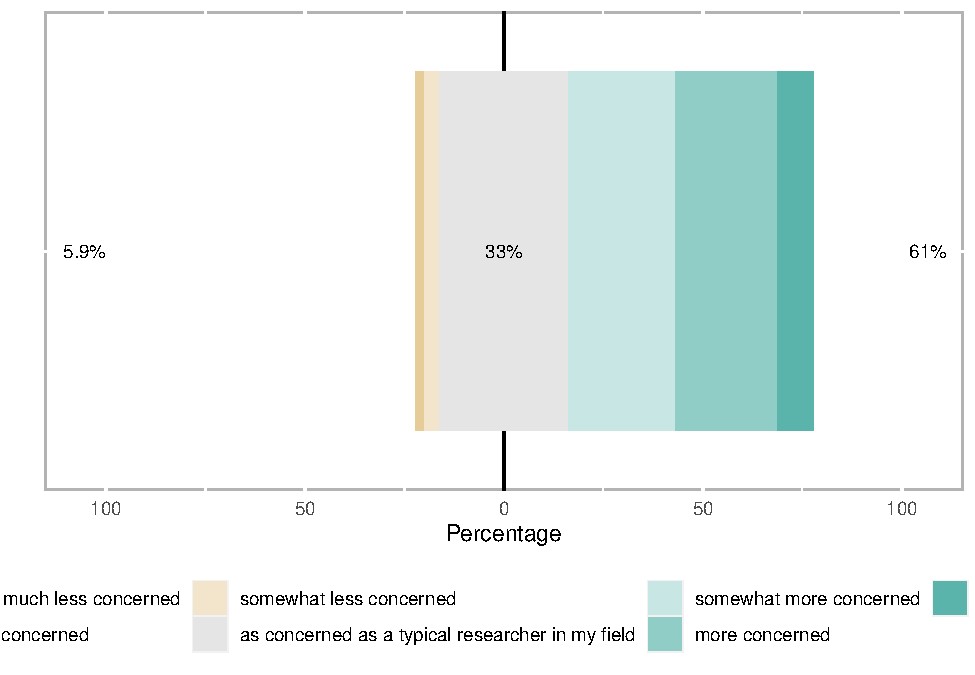
\includegraphics{manuscript_files/figure-latex/unnamed-chunk-3-1.pdf}

\hypertarget{survey-results}{%
\subsection{Survey results}\label{survey-results}}

Respondents generally agreed that studies that analyze preexisting observational datasets are trustworthy (72\%) and reproducible (79\%) (Figure 1A). At the same time, many agreed that a study using an ECAW would be more trustworthy\footnote{The survey defined trustworthy as: ``meaning that the results and conclusions of the publications are valid, reliable, rigorous, and accurate. That they merit trust.''} (70\%) and more reproducible\footnote{The survey defined reproducible ``in the sense that other researchers re-analysing the data with the same research question would produce similar results.''} (69\%) compared to a typical study using preexisting observational data (Figure 1B).

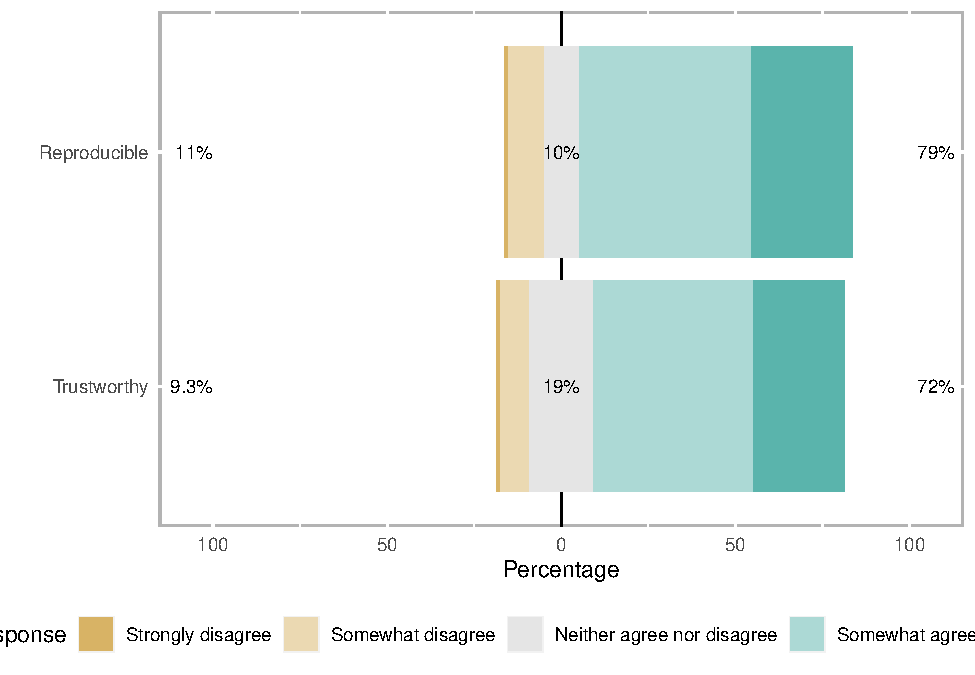
\includegraphics{manuscript_files/figure-latex/unnamed-chunk-6-1.pdf}

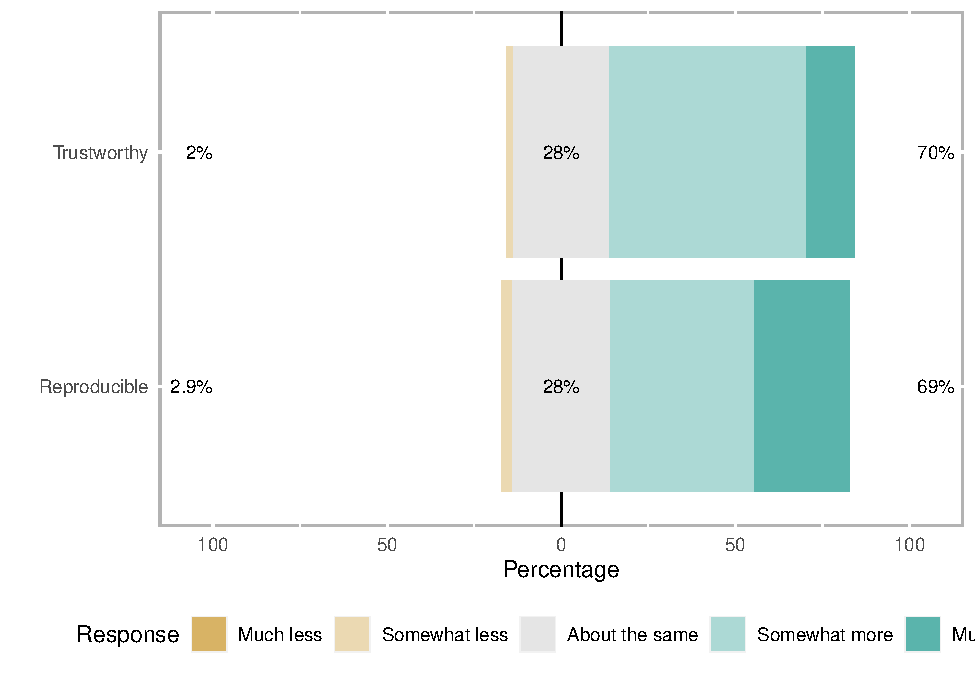
\includegraphics{manuscript_files/figure-latex/unnamed-chunk-7-1.pdf}

Almost all respondents answered that they use both exploratory (95\%) and confirmatory (92\%) analyses at least sometimes (Figure 2A-B). About half reported sharing their analysis scripts never or almost never (20\%), or sometimes (32\%) (Figure 2C). Over half reported preregistering their studies never or almost never (38\%), or sometimes (27\%) (Figure 2D). 79\% reported that they never or almost never blind the data analyst (Figure 2E).

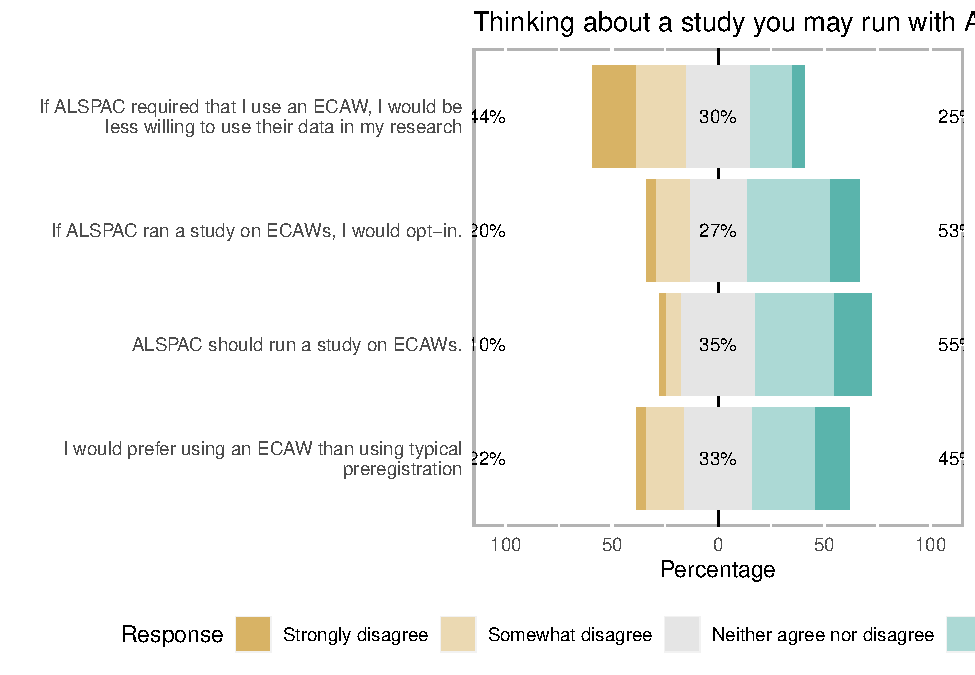
\includegraphics{manuscript_files/figure-latex/unnamed-chunk-10-1.pdf}

25\% of respondents agreed (versus 44\% who disagreed) that they would be less willing to use ALSPAC data if they were required to use an ECAW (Figure 3). 53\% agreed (20\% disagreed) that they would opt-in if ALSPAC ran a study on ECAWs. 55\% agreed (10\% disagreed) that ALSPAC should run a study on ECAWs. 45\% agreed (22\% disagreed) that they would prefer using an ECAW than using typical preregistration.

\begin{verbatim}
## Warning in likert(alspac_plot_data): Variable I would be
## less willing to use is not a factor.
\end{verbatim}

\begin{verbatim}
## Warning in likert(alspac_plot_data): Variable I would opt in is not a factor.
\end{verbatim}

\begin{verbatim}
## Warning in likert(alspac_plot_data): Variable ALSPAC should
## run a study is not a factor.
\end{verbatim}

\begin{verbatim}
## Warning in likert(alspac_plot_data): Variable I would
## prefer ECAW is not a factor.
\end{verbatim}

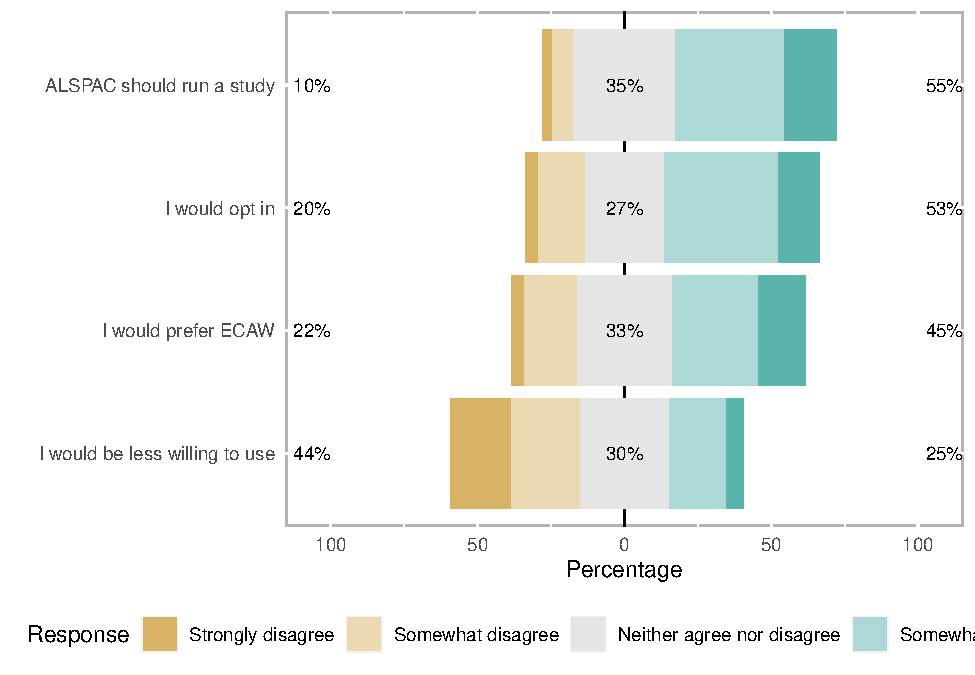
\includegraphics{manuscript_files/figure-latex/unnamed-chunk-13-1.pdf}

Address the concerns from the open-ended questions {[}transfer to right side of table 1{]}. For some research questions, the subset method may not work. In which case, a larger sample could be provided, or better yet, a synthetic dataset could be provided. The time burden is likely more than when not preregistering, but efforts can be made to minimize it. One study comparing \textasciitilde120 analyses found that an ECAW-like workflow took similar effort to preregistration (although that was for a relatively clean dataset---whereas prereg may take longer if the dataset is a mess; or viceversa). The concern that analysis would need to change after writing an ECAW is not a big deal---having the ECAW written could provide evidence that the changes were small. This is often raised as an issue in preregistraiton as well, but is acceptable or encouraged when it makes sense to do so. Finally the issue that ECAW would not work for situations where researchers are reanalyzing a dataset they already have is true, and it simply would not be possible in this situation (in which case, the researcher would not be requesting that data again anyhow, so it's beside the point).

\hypertarget{exploratory-analyses}{%
\subsection{Exploratory analyses}\label{exploratory-analyses}}

\hypertarget{discussion}{%
\section{Discussion}\label{discussion}}

Are ECAWs applicable 1? Yes. In short, ECAWs could be implemented in many cases. Many respondents use software that would allow for the ECAW format (R, ?Stata?), although some use software where this would be more difficult (SPSS, ?SAS?). Most have experience publishing relevant articles, so are familiar with the process. And most respondents also run studies that contain confirmatory analyses.

Are ECAWs applicable 2? Yes. Current methods to improve rigour and reproducibility are underused (sharing analysis scripts, blinding data analysts, preregisteration).

How biased are these results? Many that are earlier in their career based on \# of publications. Also many are more concerned than others about reproducibility. So this may, unsurprisingly, be a somewhat biased sample. Although the 10\% response rate was quite good.

Should we ALSPAC (or another org) run a study? Probably.

How would ECAWs be implemented? Would ALSPAC or the org check whether they run. Where would the be uploaded. Would the primary outcomes need to be clearly identified in the output. These would depend on the organization running such an experiment / workflow.

\hypertarget{acknowledgements}{%
\section{Acknowledgements}\label{acknowledgements}}

\newpage

\hypertarget{references}{%
\section{References}\label{references}}

\hypertarget{refs}{}
\begin{CSLReferences}{0}{0}
\end{CSLReferences}


\end{document}
